\normaltrue
\correctiontrue

%\UPSTIidClasse{11} % 11 sup, 12 spé
%\newcommand{\UPSTIidClasse}{12}

\exer{Mouvement RT  $\star$ \label{C1:05:05:PFD}}
\setcounter{question}{0}\UPSTIcompetence[2]{B2-14}
\UPSTIcompetence[2]{C1-05}
\index{Compétence B2-14}
\index{Compétence C1-05}
\index{Principe fondamental de la dynamique}
\index{PFD}
\index{Mécanisme à 1 rotation et 1 translation}
\ifcorrection
\else
\marginnote{\textbf{Pas de corrigé pour cet exercice.}}
\fi

\ifprof
\else
Soit le mécanisme suivant. On a $\vect{AB}=\lambda(t)\vect{i_1}$. De plus :
\begin{itemize}
\item $G_1$ désigne le centre d'inertie de \textbf{1} et $\vect{AG_1}=L_1\vect{i_1}$, on note $m_1$ la masse de \textbf{1}; %et $\inertie{G_1}{1}=\matinertie{A_1}{B_1}{C_1}{0}{0}{0}{\bas{1}}$; 
\item $G_2=B$ désigne le centre d'inertie de \textbf{2}, on note $m_2$ la masse de \textbf{2}.% et $\inertie{G_2}{2}=\matinertie{A_2}{B_2}{C_2}{0}{0}{0}{\bas{2}}$.
\end{itemize}


Un moteur électrique positionné entre \textbf{0} et \textbf{1} permet d'actionner le solide \textbf{1}.
Un vérin électrique positionné entre \textbf{1} et \textbf{2} permet d'actionner le solide \textbf{2}

L'accélération de la pesanteur est donnée par $\vect{g}=-g\vect{j_0}$.

\begin{center}
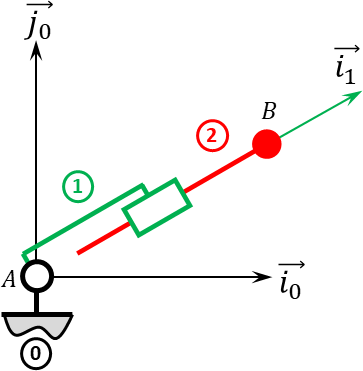
\includegraphics[width=\linewidth]{05_RT_01}
\end{center}
\fi

\question{Réaliser le graphe d'analyse en faisant apparaître l'ensemble des actions mécaniques.}
\ifprof
\begin{center}
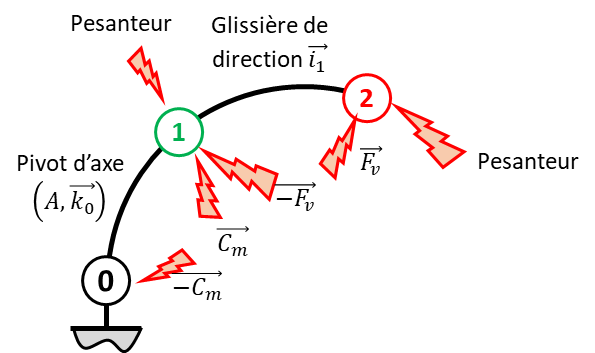
\includegraphics[width=\linewidth]{05_RT_01_cor}
\end{center}

\else
\fi

\question{Proposer une démarche permettant de déterminer les loi de mouvement de \textbf{1} et de \textbf{2} par rapport à $\rep{0}$.}
\ifprof
\begin{itemize}
\item On isole \textbf{\{1\}}. On réalise un théorème de la résultante dynamique en projection sur $\vect{i_1}$ :
$ \vectf{1}{2}\cdot \vect{i_1} + \vectf{F_v}{2}\cdot \vect{i_1} + \vectf{\text{Pes}}{2}\cdot \vect{i_1} = \vectrd{2}{0}\cdot \vect{i_1}$.
\item On isole \textbf{\{1+2\}}. On réalise un théorème du moment dynamique en $A$ en projection sur $\vect{k_0}$ :
$ \vectm{A}{0}{1}\cdot \vect{k_0} 
+ \vectm{A}{\text{Mot}}{1}\cdot \vect{k_0} 
+ \vectm{A}{\text{Pes}}{2}\cdot \vect{k_0}
+ \vectm{A}{\text{Pes}}{1}\cdot \vect{k_0} = \vectmd{A}{2}{0}\cdot \vect{k_0}+\vectmd{A}{1}{0}\cdot \vect{k_0}$.
\end{itemize}
\else
\fi


\ifprof
\else
\begin{flushright}
\footnotesize{Corrigé  voir \ref{C1:05:05:PFD}.}
\end{flushright}%
\fi